\section{Analysis: Why VLMs Don't Work Well?}

\subsection{Limited Spatiotemporal Cognition}
Despite significant advances in VLMs, their ability to understand and reason about motion, spatial relationships, and temporal coherence remains fundamentally underdeveloped ~\cite{chen2024we, apollo}. Chain of Thought (CoT)~\cite{wei2022chain} is widely employed as a method to improve accuracy through step-by-step reasoning. We showcase a comparison between CoT and DO in ~\cref{fig:cot_vs_do}. Overall, there is no indication of a large advantage of CoT over all evaluated models. Upon deeper exploration of the CoT reasoning of some models, we observe that the reasoning process was primarily flawed in the following ways: irrelevant information and arriving at conclusions that are inconsistent with the reasoning process. Larger models exhibited strategies that would be similar to how a human processes spatiotemporal information, but the resulting execution falls short of human performance. This demonstrates a disconnect between its visual and linguistic knowledge. We provide examples of this behavior in the supplement. 

\begin{figure}
    \centering
    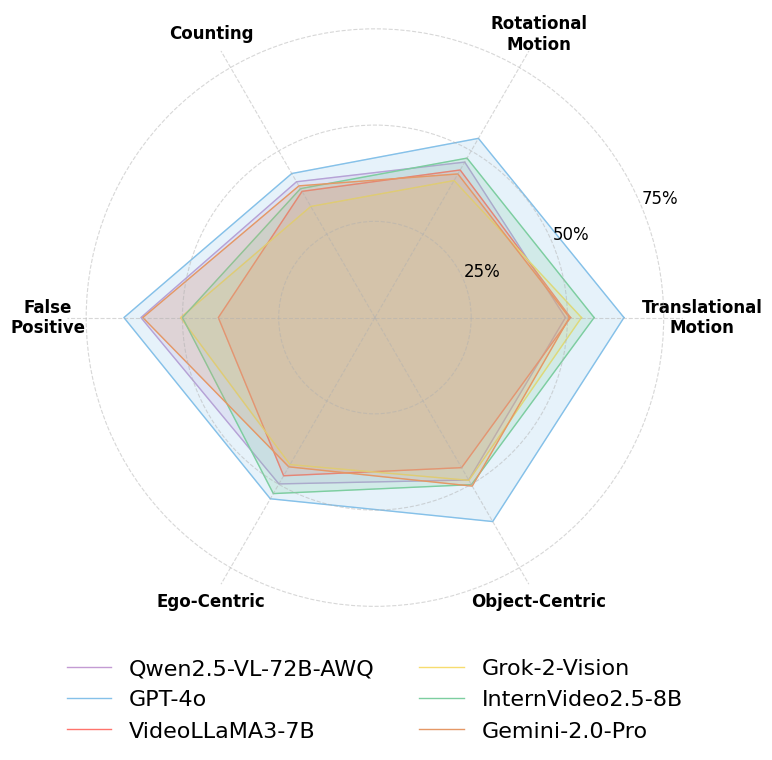
\includegraphics[width=1\linewidth]{figures/radar_plot.png}
    \caption{Model Accuracy Across Real Scene Question Categories of top-performing VLMs.}
    \label{fig:radar_plot}
    \vspace{-0.3cm}
\end{figure}

\begin{figure}
    \centering
    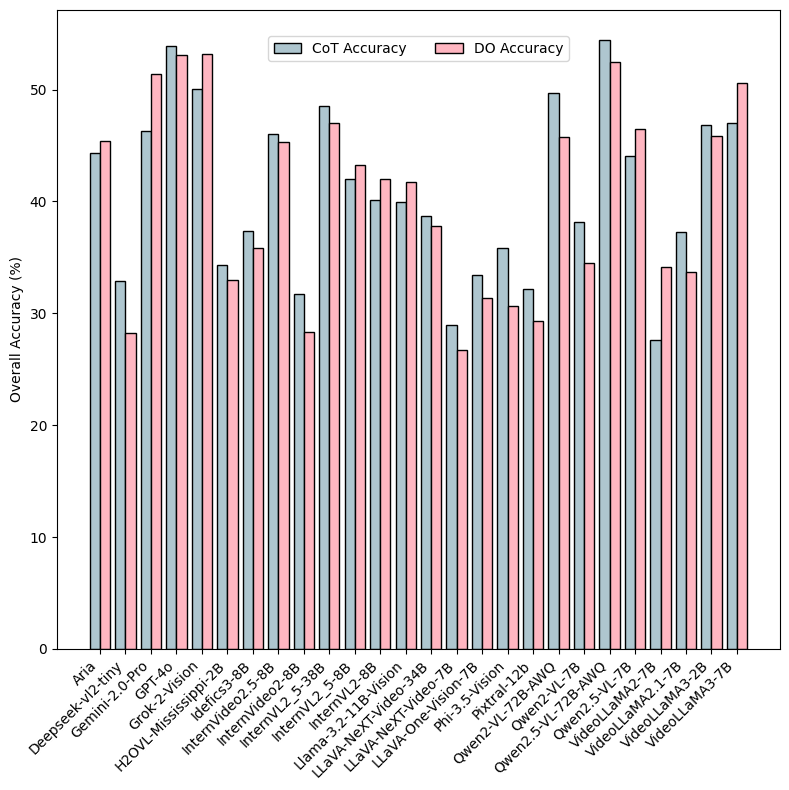
\includegraphics[width=\linewidth]{figures/cot_vs_do.png}
    \caption{\textbf{Comparison of CoT and DO Accuracy Across Models.} Accuracy comparison between Chain-of-Thought (CoT) and Direct Output (DO) prompting across VLMs.}
    \label{fig:cot_vs_do}
    \vspace{-0.5cm}
\end{figure}

\subsection{Deficiencies in Spatiotemporal Labeling}
Another avenue of exploration we undertook is to understand the richness of spatiotemporal labels in popular SFT VLM datasets. Typically, video captioning occurs at the 'scene' level, lacking fine-grained temporal, spatial, and object-level details. We performed an extensive analysis, encompassing over 2 million samples~\cite{chen2024sharegpt4video, cui2025comprehensive, 2023videochat, li2023mvbench, zhang2024llavanext-video}. We performed this analysis through string-matching of spatiotemporal descriptors related to directionality, translational motion, rotation, and perspective shifts and provide the overall results in ~\cref{fig:sft_ds}. We then performed a manual finegrained evaluation of the ShareGPT4Video dataset \cite{chen2024sharegpt4video} which we found had the highest density of spatiotemporal datasets. We found that from a sample of 100 labels that were detected as spatiotemporal, less than 10\% of them were judged as accurate upon human evaluation. This result underscores the inadequacy of current dense captioning approaches, which frequently generate spatiotemporal descriptors without capturing precise motion dynamics. We provide more detailed analysis and explanations in the supplement.
% The deficiency of comprehensive spatiotemporal annotations extends to the text-to-video (T2V) domain as well \cite{liu2023fetv,2502.02492}. These models struggle to produce temporally coherent and contextually accurate videos, often exhibiting unnatural motions or inconsistent object interactions that undermine realism. \cite{Meta2025VideoJAM, Luo2025EnhanceAVideo, DirectorLLM2024, PhysGen2024} Besides utilizing labels, recent research efforts have aimed to interpret and visualize spatial breakdowns in Vision-Language Models (VLMs), focusing on compositionality and scene structure representation throughout videos. Additionally, methods have been proposed to enhance VLMs by incorporating structured representations, such as scene graphs, or a mixture of visual prompting and intermediate representations \cite{yang2023setofmark, Zhang_2024_CVPR, Wan2024ContrastiveRG}, to improve their comprehension of spatial relationships within scenes \cite{ramakrishnan2025does, Tang2024SparkleMB, yang2024think}.

\begin{figure}[b]
    \centering
    % Replace 'example-image' with your image file name (e.g., 'myfigure.png')
    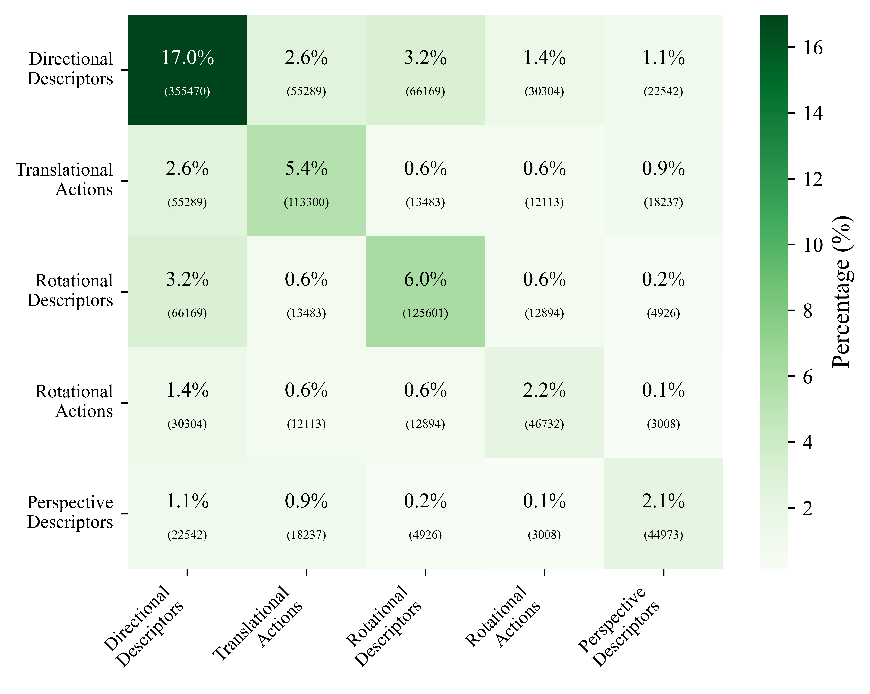
\includegraphics[width=0.5\textwidth]{figures/sft_ds_analysis.pdf}
    \caption{\textbf{Heatmap of Occurances of Spatial-Temporal Terms in popular video SFT datasets.}}
    \label{fig:sft_ds}
\end{figure}

\section{Probing Future Solutions}
To probe promising future solutions for enhancing spatiotemporal video understanding, we propose two approaches that address some of the shortcomings of current state-of-the-art VLMs: fine-tuning a VLM on data-rich in spatiotemporal actions and the other leveraging 4D reconstruction and feature fields jointly with a VLM. SFT refines the model’s abilities by training on datasets that contain temporally and spatially rich actions and interactions. By integrating structured visual representations and targeted fine-tuning, these approaches enhance video-language models’ ability to interpret motion. The second method lifts the feature space of VLMs into a temporally coherent 4D feature field, providing structured scene representations that improve motion and spatial reasoning in the stage of decoding and inference.

\paragraph{Spatial-Temporal SFT}
We evaluate on a subset split of the real dataset by splitting the real-world dataset into a training and testing split (80\% / 20\%) and we try settings using synthetic/real/both for training. We conducted the experiments using Qwen 2VL (7B) and Qwen 2.5VL (7B) through LLama-Factory~\cite{zheng2024llamafactory}, and compared the performance before and after supervised fine-tuning in~\cref{tab:sft}. The results demonstrated an improvement in accuracy in spatiotemporal reasoning, suggesting that performance gains can be obtained through targeted training. However, the addition of synthetic data does not necessarily increase performance over using real data alone, suggesting the importance of synthetic data quality.

% \paragraph{4D Feature Fields Reconstruction}
% Recent advancements in the area of 3D/4D reconstruction, such as Feature4X~\cite{zhou2025feature4x}, have demonstrated notable improvements in VLM performance for visual question answering (VQA) tasks by injecting the 4D scene representation in the feature space at the VLM inference stage. Motivated by these promising results, we explore to inject the spatiotemporal awareness following their 4D feature lifting methodology to evaluate its effectiveness on enhancing the spatiotemporal understanding of the InternVideo2-8B~\cite{wang2024internvideo2} model,testing on the subset of \texttt{VLM4D} including all 50 videos from DAVIS 2016 dataset~\cite{perazzi2016benchmark}. 

% Our experiments involved comparative inference evaluations across three distinct input modalities: original 2D videos, reconstructed global view RGB videos (4D ), and reconstructed global feature fields. As illustrated in Table~\ref{tab:4D_recon_results}, the highest accuracy was consistently obtained using the reconstructed semantic feature fields, highlighting the advantages of structured 4D scene representations. These findings confirm that global 4D feature field reconstruction substantially enriches contextual understanding while bypassing the affect by the artifact from RGB rendering during 4D reconstruction. However, this method is not a generalizable method but a per-scene optimization post-processing method, thereby significantly time-consuming.
% \paragraph{4D Feature Fields Reconstruction}
% Recent advancements in the area of 3D/4D reconstruction, such as Feature4X~\cite{zhou2025feature4x}, have demonstrated notable improvements in VLM performance for visual question answering (VQA) tasks by injecting the 4D scene representation in the feature space at the VLM inference stage. Motivated by these promising results, we explore to inject the spatiotemporal awareness following their 4D feature lifting methodology to evaluate its effectiveness on enhancing the spatiotemporal understanding of the InternVideo2-8B~\cite{wang2024internvideo2} model,testing on the subset of \texttt{VLM4D} including all 50 videos from DAVIS 2016 dataset~\cite{perazzi2016benchmark}. Our experiments involved comparative inference evaluations across three distinct input modalities: original 2D videos, reconstructed global view RGB videos (4D), and reconstructed global 4D feature field. As illustrated in~\cref{tab:4D_recon_results}, the highest accuracy was consistently obtained using the reconstructed semantic feature fields, highlighting the advantages of structured 4D scene representations. These findings confirm that global 4D feature field reconstruction substantially enriches contextual understanding while bypassing the affect by the artifact from RGB rendering during 4D reconstruction. However, this method is not a generalizable method but a per-scene optimization post-processing method, thereby significantly time-consuming.

\paragraph{4D Feature Fields Reconstruction} Recent advances in 3D/4D reconstruction methods, such as Feature4X~\cite{zhou2025feature4x}, have significantly enhanced Vision-Language Model (VLM) performance on visual question answering (VQA) tasks by integrating structured 4D scene representations into the model’s inference stage. Inspired by these promising results, we investigate incorporating spatiotemporal awareness into the InternVideo2-8B model~\cite{wang2024internvideo2}, employing the 4D feature lifting strategy proposed by Feature4X. To assess this approach, we evaluate performance on a subset of the \texttt{VLM4D} benchmark, specifically leveraging all 50 videos from the DAVIS 2016 dataset~\cite{perazzi2016benchmark}.
Our experimental evaluation compares the inference results across three distinct input modalities: original 2D videos, reconstructed global-view RGB videos (4D), and reconstructed global semantic feature fields. As demonstrated in Table~\ref{tab:4D_recon_results}, the highest accuracy consistently results from the reconstructed semantic feature fields, highlighting the clear advantages of structured 4D representations. These findings confirm that global 4D feature field reconstruction enhances contextual understanding and mitigates artifacts associated with RGB rendering during reconstruction. However, the current approach requires per-scene optimization as a post-processing step, limiting its generalizability and making it computationally intensive.

\begin{table}[t]
    \centering
    \renewcommand{\arraystretch}{1.2}
    \begin{tabular}{l|cc}
        \toprule
        \textbf{Model} & \textbf{FF} & \textbf{MC} \\
        \midrule
        \rowcolor[HTML]{e1f0f5} \textit{Original Model} & \phantom{-} & \phantom{-} \\
        Qwen 2VL (7B) & 31.9 & 38.3 \\
        Qwen 2.5VL (7B) & 31.6 & 43.4 \\
        % Video-LLama3 (3B) & - & - \\
        \midrule
        \rowcolor[HTML]{e1f0f5} \textit{Finetuned Model} & & \\
        Qwen 2VL (7B) (R) & \textbf{50.7} & 53.5 \\
        Qwen 2VL (7B) (S) & 38.9 & 41.0 \\
        Qwen 2VL (7B) (R+S) & 49.7 & 52.8 \\
        Qwen 2.5VL (7B) (R) & 48.9 & \textbf{56.3} \\
        Qwen 2.5VL (7B) (S) & 35.4 & 42.0 \\
        Qwen 2.5VL (7B) (R+S) & 39.2 & 48.3 \\
        % Video-LLama3 (3B) (R) & - & - \\
        % Video-LLama3 (3B) (R+S) & - & - \\
        \bottomrule
    \end{tabular}
    \caption{\textbf{SFT on Spatial-Temporal Datasets.} MC and FF refer to multiple-choice and freeform accuracy, respectively. R means SFT using the real-world dataset, S denotes the synthetic dataset, R+S represents using both.}
    \label{tab:sft}
\end{table}

\begin{table}[t]
    \centering
    \renewcommand{\arraystretch}{1.2}
    \begin{tabular}{l|cc}
        \toprule
        \textbf{Input Modality} & \textbf{Accuracy} \\
        \midrule
        \rowcolor[HTML]{e1f0f5} \textit{Chain of Thought Response} & \phantom{-} & \phantom{-} \\
        Original 2D Video & 36.0 \\
        Global View Video & 32.7 \\
        Global Feature Field & \textbf{37.4} \\
        \midrule
        \rowcolor[HTML]{e1f0f5} \textit{Direct Output Response} & & \\
        Original 2D Video & 24.3 \\
        Global View Video & 23.8 \\
        Global Feature Field & \textbf{29.0} \\
        \bottomrule
    \end{tabular}
    \caption{\textbf{InternVideo2 Accuracy with 4D Reconstruction.} Comparison of InternVideo2 accuracy given different input modalities from the same dataset.}
    \label{tab:4D_recon_results}
    \vspace{-0.3cm}
\end{table}

% \begin{table*}[h]
%     \centering
%     \renewcommand{\arraystretch}{1.2}
%     \begin{tabular}{lccc}
%         \toprule
%         \textbf{Model} &  \makecell{\textbf{Synthetic (CoT)}}  & \makecell{\textbf{3rd Person}\\ \textbf{Perspective (CoT)}} &  \makecell{\textbf{1st Person}\\ \textbf{Perspective (CoT)}} \\
%         \midrule
%         \rowcolor[HTML]{F5E8DC} ProLong (8B) & 20.4 / 25.4 & \textbf{28.4} / \textbf{30.1} & 17.0 / 17.1 \\
%         MegaBeam-Mistral (7B) & 512K & 19.8 & \textbf{18.3} \\
%         Meta-Llama-3.1 (8B) & 128K & 17.3 & 16.4 \\
%         Mistral-Nemo (12B) & 128K & 13.6 & 0.4 \\
%         \midrule
%         Jamba-1.5-Mini (12B/52B) & 256K & 27.2 & 28.0 \\
%         Meta-Llama-3.1 (70B) & 128K & 42.0 & 25.0 \\
%         Gemini-1.5-Pro & 2M & 24.7 & 38.8 \\
%         GPT-4o & 128K & 55.6 & 58.4  \\
%         \bottomrule
%     \end{tabular}
%     \caption{\textbf{Big Results Evaluation of Various VLLMs}}
% \end{table*}